
\documentclass[letterpaper,twocolumn,10pt]{article}
\usepackage{usenix2019_v3}

% to be able to draw some self-contained figs
\usepackage{tikz}
\usepackage{amsmath}
\usepackage{pgfplots}

% inlined bib file
\usepackage{filecontents}

\begin{document}
%-------------------------------------------------------------------------------

%don't want date printed
\date{}

% make title bold and 14 pt font (Latex default is non-bold, 16 pt)
\title{\Large \bf General Matrix Multiplication (GEMM) with OpenMP}

%for single author (just remove % characters)
\author{
{\rm Robert Geil}\\
University of California, Los Angeles
} % end author

\maketitle

%-------------------------------------------------------------------------------
\begin{abstract}
%-------------------------------------------------------------------------------
General Matrix Multiplication (GEMM) is an important problem type in many fields
of computer science and is therefore a good candidate for optimization and
parallelization. In this lab, we utilized cacheing and parallel programming with
OpenMP to speedup the multiplication of large matricies as compared to a na\"{i}ve 
approach, reaching roughly 110 Gigaflops at peak
\end{abstract}


%-------------------------------------------------------------------------------
\section{Introduction}
%-------------------------------------------------------------------------------

Matrix multiplication is a problem that arises in many areas of computer science,
from image processing to AI. As such, by optimizing this one problem, many slow
processes can be sped up and take advantage of the compute resources in the
many core era. To that end, we would like to apply both parallelism through
OpenMP as well as improve cache performance by limiting cache misses. To achieve
these goals, we will use OpenMP's preprocessor statements for parallelism, and
use loop permutations to improve cache hit rates.

%-------------------------------------------------------------------------------
\section{Machine Specifications}
%-------------------------------------------------------------------------------

The machine for which the code was optimized is an Amazon Web Services (AWS)
\textit{m5.2xlarge} virtual machine. This machine has 8 virtual CPUs, each of
which supports 2 threads via Intel's Hyperthreading technology. The processor is
clocked at %TODO GHz, and contains %TODO Kb L1, Kb L2 and Kb L3 cache.

%-------------------------------------------------------------------------------
\section{Solution Approach}
%-------------------------------------------------------------------------------
For this problem, we took two approaches. First was a \textit{parallel} approach, where
we only used loop reordering and OpenMP to improve the performance of the code.
In the other approach, \textit{parallel blocked}, we both used OpenMP for parallelization
and used a technique called \textit{loop tiling} to extract more performance from
the cache.
\subsection{OpenMP}
To integrate OpenMP into the solution, we used the preprocessor directives portion
of OpenMP. The one most heavily utilized was the parallel for loop, as seen below
\begin{verbatim}
#pragma parallel for private(j, k)
for(int i = 0; ...){
\end{verbatim}
This, placed just outside the outermost for loop of the multiplication split the
work among a number of threads, each taking a portion of the multiplication.
Here private variables were used to prevent the threads from overwriting each
other's $j$ and $k$ variables as they proceeded through the inner loops. In addition,
for the \textit{parallel blocked} implemention, additional variables for the blocks
were added to the private list, as well as a \textit{schedule(static, 32)} which was
found to improve performance by scheduling larger blocks to work at the same time.
\subsection{Loop Ordering}
The na\"{i}ve approach to matrix multiplication uses a triple for loop first iterating
over $i$, then $j$ and finally $k$
\begin{verbatim}
for(int i = 0; i<I; i++){
  for(int j = 0; j<J; j++){
    for(int k = 0; k<K; k++){
      c[i][j] = a[i][k]*b[k][j];
    }
  }
}
\end{verbatim}
However, because of how matrices are laid out in memory, this turns out to be a 
quite inefficient approach. Since arrays in C/C++ are stored in row-major order,
increasing k frequently as part of the innermost loop means that matrix $b$ cannot
be effectively cached, as each time a whole new row must be read from main memory.
To improve on this, we can reorder the loops without changing the semantics of the
program as follows
\begin{verbatim}
  for(int i = 0; i<I; i++){
    for(int k = 0; k<K; k++){
      for(int j = 0; j<J; j++){
        c[i][j] = a[i][k]*b[k][j];
      }
    }
  }
  \end{verbatim}
With this reordering, we see that the value read from a can be cached for $J$ 
iterations, while the values read from b and stored to c exhibit spatial
locality, as they are being read linearly from memory.
\subsection{Loop Tiling}
With a traditional matrix multiplication of matricies 
%-------------------------------------------------------------------------------
\section{Results}
%-------------------------------------------------------------------------------
\begin{figure}
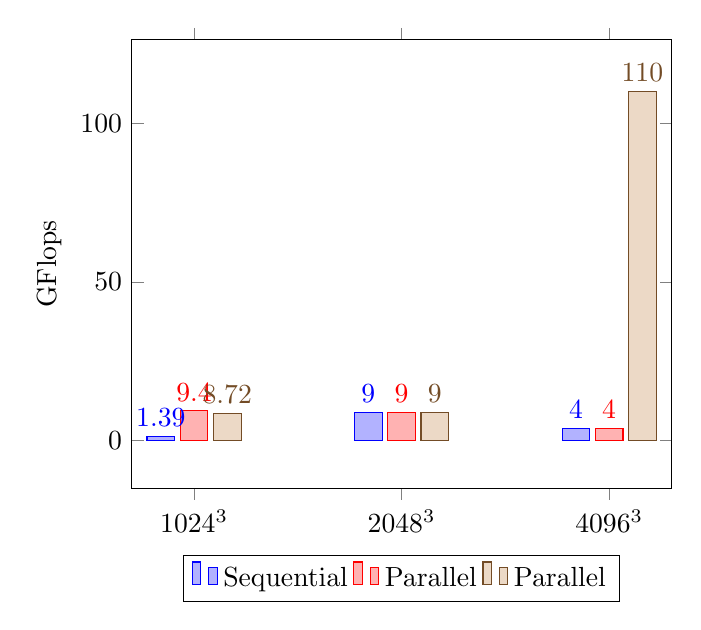
\begin{tikzpicture}
  \begin{axis}[
      ybar,
      enlargelimits=0.15,
      legend style={at={(0.5,-0.15)},
        anchor=north,legend columns=-1},
      ylabel={GFlops},
      symbolic x coords={$1024^3$,$2048^3$,$4096^3$},
      xtick=data,
      nodes near coords,
      nodes near coords align={vertical},
      ]
      \addplot coordinates {($1024^3$,1.3872) ($2048^3$,9) ($4096^3$,4)};
      \addplot coordinates {($1024^3$,9.4) ($2048^3$,9) ($4096^3$,4)};
      \addplot coordinates {($1024^3$,8.72) ($2048^3$,9) ($4096^3$,110)};
  \legend{Sequential,Parallel,Parallel}
  \end{axis}
  \end{tikzpicture}
  \caption{\label{fig:vectors} Text size inside figure should be as big as
  caption's text. }
\end{figure}
%---------------------------


Here's a typical reference to a floating figure:
Figure~\ref{fig:vectors}. Floats should usually be placed where latex
wants then. Figure\ref{fig:vectors} is centered, and has a caption
\end{document}
%%%%%%%%%%%%%%%%%%%%%%%%%%%%%%%%%%%%%%%%%%%%%%%%%%%%%%%%%%%%%%%%%%%%%%%%%%%%%%%%

%%  LocalWords:  endnotes includegraphics fread ptr nobj noindent
%%  LocalWords:  pdflatex acks